%=====================================================
%
% Variables (same scheme as the sample document)
%
%=====================================================

\def\doctype{article}

\def\emptypages{false}
\def\showparts{false}

\def\ttitlepage{titlepage.tex}
\def\ttitlepagetitletop{Claimed and Measured}
\def\ttitlepagesubtitletop{Gyro-S v2 on Real Coding Tasks, and Why the Test Needs Testing Too}
\def\ttitlepagetitlemiddle{Lab Report}
\def\ttitlepagesubtitlemiddle{Measurements of 24--26 November 2026}

\def\torganization{Independent Research}
\def\tsubmissiondate{25 November 2026}
\def\tversion{0.2}
\def\tauthor{Matthias Nott}
\def\tcontact{~}
\def\tcontactid{~}

\def\tfooterleftlabelup{Title}
\def\tfooterleftlabeldown{Author}
\def\tfooterleftup{Local Coding Agents, Report 6}
\def\tfooterleftdown{Matthias Nott}
\def\tfootermiddleup{Claims and Real Tasks}
\def\tfootermiddledown{Lab Report}
\def\tfooterrightlabelup{Date}
\def\tfooterrightlabeldown{Version}
\def\tfooterrightup{November 2026}
\def\tfooterrightdown{0.2}

\def\showtitlepage{true}
\def\showlistofs{true}
\def\showtoc{true}
\def\showlot{true}
\def\showlof{false}
\def\showloe{false}
\def\showlod{false}

\def\showreferences{true}
\def\showappendix{false}
\def\showendnotes{false}
\def\showanyglossary{false}
\def\showacronyms{false}
\def\showglossary{false}
\def\showstatic{false}
\def\showindex{false}

\def\showpageheaders{true}
\def\showpagefooters{true}
\def\showwordcount{false}
\def\showwordcountback{false}

\input{templates/cfg/zz_layout}

\setcounter{tocdepth}{2}

\usepackage[
  style=apa
, citestyle=authoryear
, backend=biber
, maxnames=3
, minnames=1
, sorting=nyt
, sortcites=true
, block=space
, safeinputenc
, natbib=true
, backref=true
, uniquename=init]{biblatex}
\DeclareLanguageMapping{american}{american-apa}
\addbibresource{Bibliography.bib}
\input{templates/cfg/zz_config_bib}

\usepackage{indentfirst}

\newcommand{\cmd}[1]{\texttt{#1}}

% Alternate row colours in every table (xcolor is loaded with the table option by the layout)
% Breathing room between tables and the running text
\setlength{\intextsep}{16pt plus 2pt minus 2pt}
\setlength{\textfloatsep}{18pt plus 2pt minus 4pt}
\setlength{\floatsep}{16pt plus 2pt minus 2pt}

\definecolor{rowtint}{gray}{0.93}
\AtBeginEnvironment{table}{\global\csname @rowcolorstrue\endcsname\rowcolors{2}{rowtint}{white}}
\newcolumntype{P}[1]{>{\raggedright\arraybackslash}p{#1}}
\setcounter{secnumdepth}{2}

\begin{document}

%=====================================================
% Title page and abstract
%=====================================================

\input{tex/\ttitlepage}

\begin{center}
\begin{minipage}{0.86\textwidth}
\section*{Abstract}

A model announcement claims Gyro-S v2 drifts 18\,\% less on held-out text, 27\,\% less on tool calls and 14\,\% less
on code than its base. We asked what the same model does as a local coding worker --- writing files that hidden tests
grade --- and measured it head-to-head against Signal 2 on one Apple M5 Max: 20 questions, 40 easy and 40 hard graded
function tasks, and five replayed real repository fixes, each run once. Accuracy is at best a draw: on the hard set
Gyro-S v2 reaches 35/40 against Signal 2's 37/40, and the easy and short sets are similar. Speed is not: Gyro-S v2 is
slower everywhere --- 899--1{,}195\,s against 490--624\,s on the hard set, 2{,}861\,s against 2{,}141\,s on the real
tasks run alone, and a much lower token rate. Stability is where they really differ: Gyro-S v2 swings from run to run
(hard 8--35/40, short 2--17/20) because it often stops early with answers missing, while Signal 2 stays inside a narrow
band (hard 30--37/40). On the real tasks Gyro-S v2 tends to be weaker (3/5, 4/5, and one incomplete run an engine stall
ended) against Signal 2's 4/5, 5/5, 3/5, 3/5 and 4/5 --- a tendency, not a clean gap, since each ran once. In memory,
Signal 2 holds about 27\,GB per instance mostly on the GPU; Gyro-S v2 keeps a smaller footprint (16--26\,GB) but a far
larger resident size (35--49\,GB), because its experts and PLE table are read from the SSD, and two instances of it
leave only about 4\,GB free. Our first run had loaded the wrong PLE table --- the base model's instead of the one this
model card pairs with --- which made Gyro-S v2 look far worse than it is; we found that after the author's question and
reran. One lesson: verify the test and the setup before a verdict.

\end{minipage}
\end{center}

\clearpage

%=====================================================
% Table of contents and list of tables
%=====================================================

\sequals{\showpageheaders}{true}{
	\pagestyle{fancy}
	\fancyhead{}
	\fancyhead[RO,LE]{\thepage}
	\fancyhead[LO]{\slshape CONTENTS}
	\fancyhead[RE]{\slshape CONTENTS}
}{}
\sequals{\showpagefooters}{true}{\fancyfoot[C]{}}{}
\pdfbookmark[-1]{\contentsname}{toc}
\tableofcontents
\addtocontents{lot}{\protect\vspace{10pt}}
\listoftables
\clearpage

\sequals{\showpageheaders}{true}{
	\pagestyle{fancy}
	\fancyhead{}
	\fancyhead[LE,RO]{\thepage}
	\fancyhead[RE]{\slshape \rightmark}
	\fancyhead[LO]{\slshape \rightmark}
}{}
\sequals{\showpagefooters}{true}{\fancyfoot[C]{\pfooter}}{}
\renewcommand{\sectionmark}[1]{\markboth{\thesection.\ #1}{\thesection.\ #1}}
\renewcommand{\subsectionmark}[1]{}
\clearpage

%=====================================================
% Body
%=====================================================

\section{Introduction}\label{sec:intro}

On 24 November the author of a fine-tune announced it with measured numbers: ``Gyro-S v2 is out. Qwen3.8-Flash-Next
(125B MoE) on one 32 GB card, now closer to the original: 18\,\% less drift on held-out text, 27\,\% less on tool
calls, 14\,\% less on code.'' Those are percentages on held-out data of the fine-tuning recipe. The question this
report asks is what the same model does in the role report 5 defined \citep{Nott-2026aa}: a local coding worker under
Claude Code \citep{Anthropic-2026aa} on the engine Strata \citep{Strata-2026aa}, writing files that hidden tests grade.
Claimed percentages and bench passes measure different things, so this report sets the claim beside what the bench
measures --- and reports a setup mistake of our own that changed the answer, because a real test only counts once the
test and the setup have been verified.

\section{Setting}\label{sec:setting}

\subsection{Model under test}

The model is Qwen3.8-Flash-Next-Gyro-S v2, quantised TQ1\_0, file 29{,}686{,}877{,}504 bytes --- the \emph{-noPLE}
GGUF.\footnote{SHA-256 \texttt{e33a245502a4ae00\allowbreak 83ac2064b019f948\allowbreak f5a2cfec6152b1dd\allowbreak 6854dd014aee66bb}, matching the model author's changelog.}
PLE (per-layer embedding) is a large lookup table that layer 1 of the model reads for every token, indexed by the
current and previous tokens (an n-gram table). It makes up about half of a full model file and stays on disk; the
\emph{-noPLE} files ship without it and load it from a separate file via \cmd{--ple-gguf}. The correct pairing for this
file is the IQ4\_NL Gyro-S table on the model card; our first run loaded the base model's Q8\_0 table instead --- see
Section~\ref{sec:first}. All results here use the author's IQ4\_NL table, loaded fresh. The runtime pack was built
fresh from the v2 file; no earlier pack was reused. This ran on Strata 0.2.21 Metal (our port branch), with MTP drafts
on. A smoke test before the bench: correct output, 92 tokens/s decode, MTP acceptance 44 of 48.

\subsection{The machine and the bench}

The machine is one Apple M5 Max with 128\,GB unified memory --- the same machine and the same bench as report 5
\citep{Nott-2026aa}: \emph{short} 20 questions with exact answers; \emph{easy} and \emph{hard} 40 function-level
Python tasks each, read-and-write only, graded by hidden tests; \emph{real} five replayed fixes from the PAI
repository (prune-dist-rerun, mirror-sync-token, worker-priority, session-move-selectors, escalate-loopstop) graded by
hidden behaviour tests, 30-minute cap per task. prune-dist-rerun is confounded by the machine (its visible test is red
before any edit; see report 5) and fails for every model here; it stays called out where it matters.

\subsection{How the head-to-head ran}\label{sec:h2h-setup}

On the night of 25/26 November both models ran the whole bench on this machine, Gyro-S v2 with the author's IQ4\_NL
PLE table and announced-no-action guard cap 6 (the corrected setup), Signal 2 with its default caps. Four phases ran in
sequence: \textbf{A} Signal 2, one instance; \textbf{B} Gyro-S v2, one instance; \textbf{C} Signal 2, two instances in
parallel; \textbf{D} Gyro-S v2, two instances in parallel. During each phase the other model's servers were stopped, so
no run shared its machine with a foreign engine. One rep per set per instance (keys h2h-s2-single, h2h-g2-single,
h2h-s2-dualA/B, h2h-g2-dualA/B). Signal 2's solo numbers are also its own reference runs from report 5; where a run was
loop-stopped after the shown number of correct writes (the guard fired on unchanged rewrites of finished files), the
passes stand and the run did not finish cleanly --- noted in the tables.

\section{Results: head-to-head}\label{sec:results}

\subsection{Pass rates}\label{sec:h2h-pass}

Table~\ref{tab:h2h} is the night's data: passed tasks and wall time per set, one rep per cell. In the dual phases each
instance ran the whole bench against itself; the two instances of a phase overlap, so their wall times differ (each
carries the other's load unevenly).

\begin{table}[H]
\centering
\small
\caption{Head-to-head, one rep per run: passed tasks and wall time per set}\label{tab:h2h}
\begin{tabular}{lrrrr}
\toprule
Run & short (20) & easy (40) & hard (40) & real (5) \\
\midrule
A: Signal 2, single & 16, 60\,s & 39, 174\,s & 37, 490\,s$^{a}$ & 4, 2{,}141\,s \\
B: Gyro-S v2, single & 2, 28\,s & 39, 536\,s$^{a}$ & 11, 170\,s & 3, 2{,}861\,s \\
C: Signal 2, instance 1 & 16, 84\,s & 37, 252\,s & 31, 540\,s$^{a}$ & 3, 4{,}532\,s \\
C: Signal 2, instance 2 & 18, 78\,s & 39, 202\,s & 32, 624\,s$^{a}$ & 4, 4{,}775\,s \\
D: Gyro-S v2, instance 1 & 15, 179\,s & 38, 737\,s & 35, 1{,}195\,s & incomplete$^{b}$ \\
D: Gyro-S v2, instance 2 & 17, 133\,s & 36, 854\,s & 27, 899\,s & incomplete$^{b}$ \\
\bottomrule
\end{tabular}
\par\smallskip{\footnotesize\raggedright $^{a}$ Run loop-stopped after the shown number of correct writes (the guard fired on unchanged rewrites of finished files); the passes stand, the run did not finish cleanly. $^{b}$ Both real series of phase~D were stopped by the harness watchdog after 15 minutes without worker activity and wrote an empty result; recovered outcomes are in Table~\ref{tab:h2h-real} and Section~\ref{sec:h2h-fault}. \par}
\end{table}

Figure~\ref{fig:h2h-pass} is the same numbers as shares, so accuracy can be read at a glance. It supports finding (a):
accuracy is at best a draw --- Gyro-S v2's best hard score (35/40, instance~1 of phase~D) sits just below Signal 2's
best (37/40), and the easy set is close for both (36--39/40). It also shows finding (c): Gyro-S v2's bars swing hard
from run to run, while Signal 2's are steady.

\begin{figure}[H]
\centering
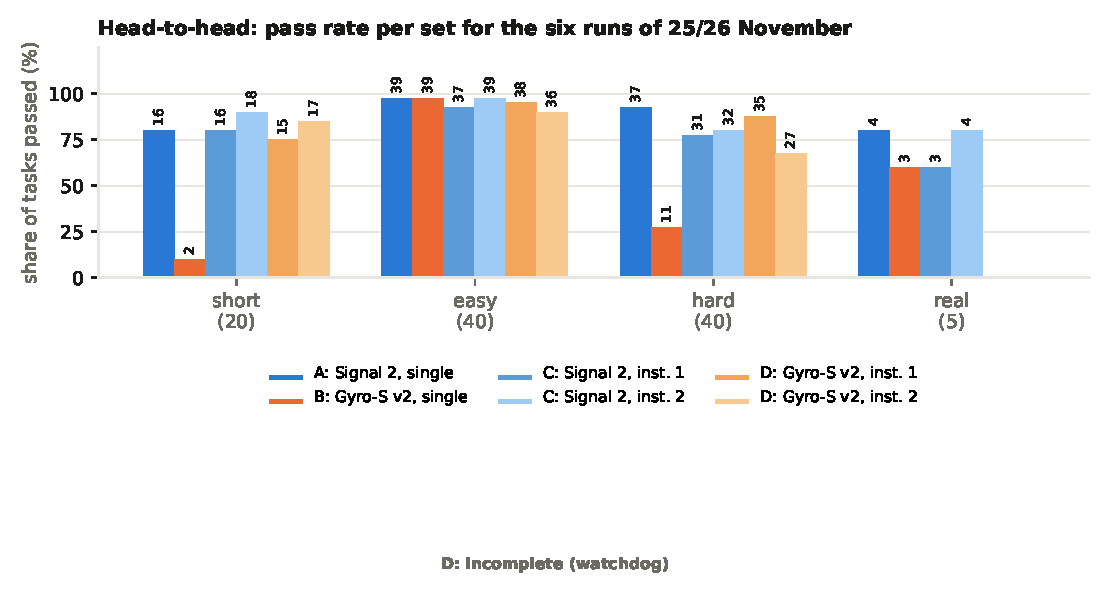
\includegraphics[width=\textwidth]{figures/fig-h2h-pass.pdf}
\caption{Pass rate per set for the six runs of Table~\ref{tab:h2h}. Orange shades are Gyro-S v2, blue shades Signal 2; darker shades are single instances, lighter the two parallel instances. Labels give passed tasks of $n$; the hatched bar marks phase~D's incomplete real series.}\label{fig:h2h-pass}
\end{figure}

\subsection{Speed}\label{sec:h2h-speed}

Gyro-S v2 is slower on every set, and the gap widens as tasks get harder. On the hard set its two dual instances took
899--1{,}195\,s against Signal 2's 490--624\,s; run alone, its real series took 2{,}861\,s against Signal 2's
2{,}141\,s. Its whole-run output rate is far lower (single hard 2.16\,tok/s against Signal 2's 31.5; single easy 2.44
against 51.2), because it spends most of its turns announcing work and stopping rather than writing --- the early-stop
pattern behind finding (c). This is why the operational choice leans toward Signal 2 (Section~\ref{sec:limits}).

\subsection{Stability}\label{sec:h2h-spread}

The hard set is where the night's real difference shows. Gyro-S v2 (author's table, cap 6) scored \textbf{11/40}
single, \textbf{35/40} and \textbf{27/40} as the two dual instances; Signal 2 scored \textbf{37}, \textbf{31} and
\textbf{32}. Gyro-S v2's early stopping --- answers never written, turns ending after announcements --- varies strongly
from run to run (its short set swings 2--17/20); Signal 2 stays inside a narrow band. That variance, not either model's
best case, is the practical difference between them: a worker whose hard-set score swings between 11/40 and 35/40
cannot be planned around, while one that stays in the 31--37 band can.

Figure~\ref{fig:h2h-spread} plots every hard-set run of this report as one dot per run, so the spread is visible rather
than summarized. It supports finding (c): Gyro-S v2's dots scatter across 8--35/40 (the two lowest were our first runs,
with the wrong PLE table --- Section~\ref{sec:first}), while Signal 2's sit in a tight column at 30--37.

\begin{figure}[H]
\centering
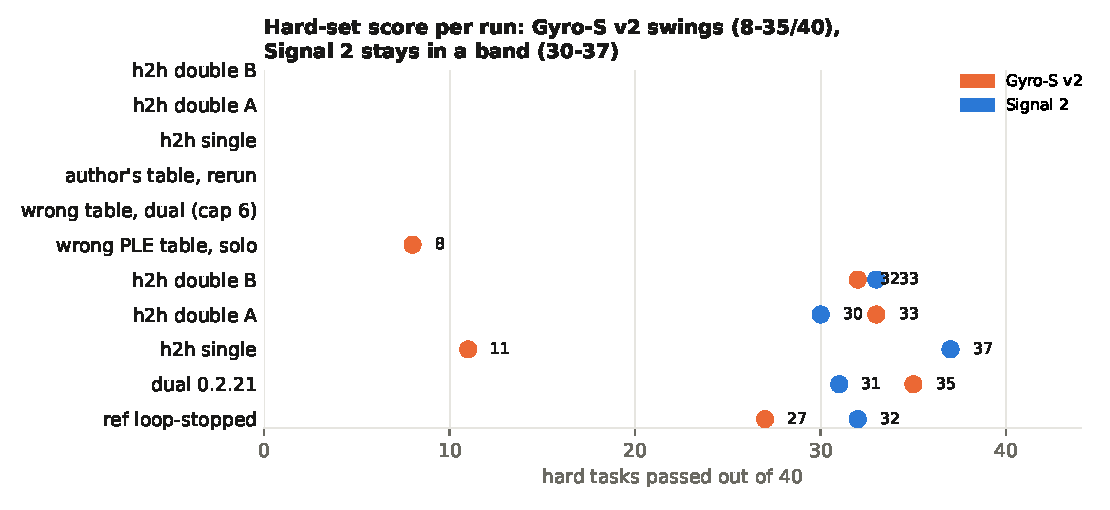
\includegraphics[width=\textwidth]{figures/fig-h2h-spread.pdf}
\caption{Hard-set score per run across all runs of this report (one rep each). Gyro-S v2's dots swing widely (8--35/40; the two lowest are the first runs with the wrong PLE table, Section~\ref{sec:first}); Signal 2 stays in a narrow band (30--37/40).}\label{fig:h2h-spread}
\end{figure}

\subsection{Real tasks}\label{sec:h2h-real}

Table~\ref{tab:h2h-real} gives the five replayed fixes per run, pass or fail with wall seconds. prune-dist-rerun fails
everywhere (the confounded task of report 5); escalate-loopstop passes for every Signal 2 run and both Gyro-S runs that
reached it.

\begin{table}[H]
\centering
\small
\caption{Real tasks, pass/fail and seconds per run}\label{tab:h2h-real}
\begin{tabular}{lrrrrr}
\toprule
Task & A: S2 single & B: G2 single & C1: S2 & C2: S2 \\
\midrule
prune-dist-rerun (confounded) & fail, 216\,s & fail, 131\,s & fail, 994\,s & fail, 1{,}855\,s \\
mirror-sync-token & pass, 138\,s & pass, 1{,}851\,s & pass, 774\,s & pass, 437\,s \\
worker-priority & pass, 1{,}220\,s & fail, 179\,s & pass, 1{,}714\,s & pass, 901\,s \\
session-move-selectors & pass, 407\,s & pass, 396\,s & pass, 664\,s & pass, 1{,}413\,s \\
escalate-loopstop & pass, 153\,s & pass, 297\,s & fail, 377\,s & pass, 162\,s \\
\midrule
Total & 4/5 & 3/5 & 3/5 & 4/5 \\
\bottomrule
\end{tabular}
\end{table}

Phase~D's real series did not produce a usable score (Section~\ref{sec:h2h-fault}). From the per-task hidden-test logs,
instance~1 got mirror-sync-token \emph{pass}, prune-dist-rerun \emph{fail} and worker-priority \emph{fail} before
stopping during task~4; instance~2 got mirror-sync-token \emph{pass} and prune-dist-rerun \emph{fail} before stopping
during task~3. These are reported as recovered outcomes, not as 0/5.

Across the usable runs Gyro-S v2 tends to be weaker on real work --- 3/5 and 4/5 run alone, plus the two incomplete
parallel runs --- against Signal 2's 4/5, 5/5 (report 5), 3/5, 3/5 and 4/5. This is finding (d): a tendency, not a
clean gap, because each ran once and one of Gyro-S v2's runs was ended by an engine stall rather than by the model.

\subsection{Memory}\label{sec:h2h-mem}

The driver recorded, at idle, under load and after each phase, the engine process's \emph{footprint} (the memory it
actually holds, including GPU-resident weights) and its \emph{resident size} (rss, which also counts file pages mapped
from disk), plus the system's free memory.

\begin{table}[H]
\centering
\small
\caption{Engine memory per instance: footprint and resident size}\label{tab:h2h-mem}
\begin{tabular}{lrrr|rrr}
\toprule
& \multicolumn{3}{c|}{Signal 2 (GiB)} & \multicolumn{3}{c}{Gyro-S v2 (GiB)} \\
\cmidrule(lr){2-4}\cmidrule(lr){5-7}
Phase & idle & load & after & idle & load & after \\
\midrule
Single & 28 & 27 & 30 & 16 & 23 & 26 \\
Double, inst.~1 & 18 & 17 & 24 & 16 & 22 & ---$^{a}$ \\
Double, inst.~2 & 17 & 25 & 27 & 16 & 22 & 26 \\
\bottomrule
\end{tabular}
\par\smallskip{\footnotesize\raggedright $^{a}$ Instance~1's engine was stopped by Strata's stall watchdog (issue~\#29) during phase~D; no after-phase sample. \par}
\end{table}

Figure~\ref{fig:h2h-mem} shows footprint against resident size per instance, at idle and under load. It supports
finding (e): reading only one number misleads about how these models fit in memory. Gyro-S v2's \emph{footprint} is
smaller than Signal 2's (16--26\,GiB against 17--30\,GiB), but its \emph{resident size} is far larger (35--49\,GiB
against 9--45\,GiB): Gyro-S v2 is a 125B MoE whose experts and whose PLE table are memory-mapped from the SSD --- those
file pages count as resident even though the process does not hold them, and the engine reads them on demand. Signal 2
keeps its weights mostly in GPU (wired) memory, so its footprint is large while its resident size is modest. The
system's free memory tracked this: phases C and D ran with only 0.1--5\,GiB free and heavy compression (up to 30\,GiB
compressed), the signature of SSD-paged MoE serving on a 128\,GB machine; two Gyro-S v2 instances leave about 4\,GB
free.

\begin{figure}[H]
\centering
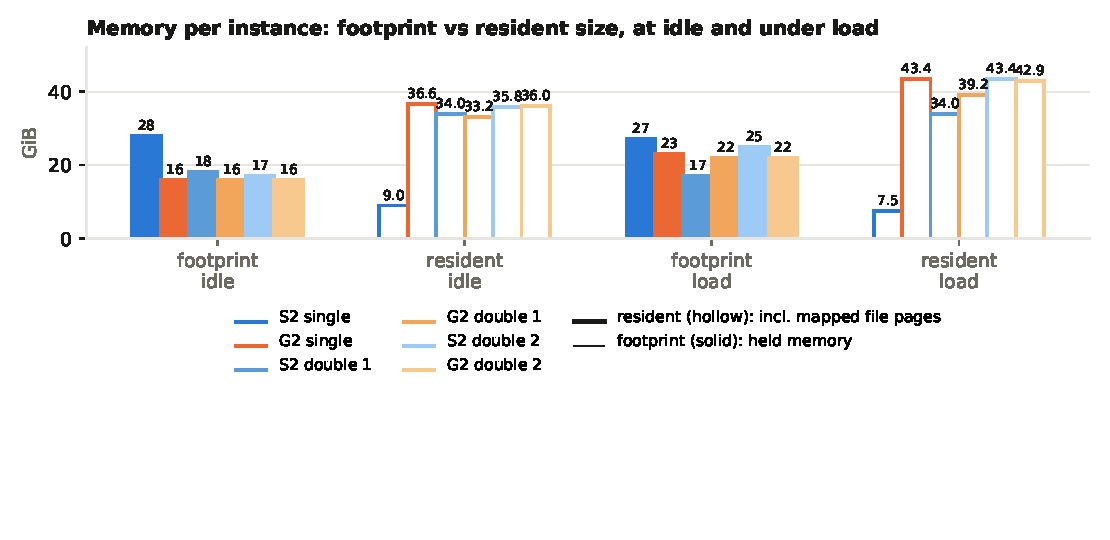
\includegraphics[width=\textwidth]{figures/fig-h2h-memory.pdf}
\caption{Memory per instance: footprint (solid, memory the process actually holds) against resident size (hollow, includes file pages mapped from disk), at idle and under load. Signal 2 in blue shades, Gyro-S v2 in orange shades; darker is single, lighter the double instances.}\label{fig:h2h-mem}
\end{figure}

\subsection{Throughput}\label{sec:h2h-thr}

Table~\ref{tab:h2h-thr} is the operational view: passed real tasks per hour. For a single instance that is
passed\,/\,wall; for a phase with two instances it is the \emph{sum} of both instances' passes over the \emph{longer}
of the two wall times --- what the machine delivered per hour. Phase~D is excluded: its real series was faulted
(Section~\ref{sec:h2h-fault}), and its function sets alone would not answer the operational question.

\begin{table}[H]
\centering
\small
\caption{Real-task throughput per phase}\label{tab:h2h-thr}
\begin{tabular}{lrrr}
\toprule
Phase & Passed real tasks & Wall (s) & Passed per hour \\
\midrule
A: Signal 2, single & 4 & 2{,}141 & 6.75 \\
B: Gyro-S v2, single & 3 & 2{,}861 & 3.77 \\
C: Signal 2, double & 7 (3 + 4) & 4{,}775 (max of 4{,}532 and 4{,}775) & 5.26 \\
D: Gyro-S v2, double & --- & --- & faulted (Section~\ref{sec:h2h-fault}) \\
\bottomrule
\end{tabular}
\end{table}

Signal 2's single instance beats its own double here: two instances pass 7 tasks but take more than twice the time of
one, so throughput drops from 6.75 to 5.26 per hour --- on this machine the real tasks saturate the shared engine, and
a second instance mostly adds waiting, not work. The whole-night totals (all four sets) are 4{,}389\,s for phase~A,
3{,}597\,s for phase~B, 10{,}106\,s for phase~C and 12{,}364\,s for phase~D.

\section{What we got wrong first, and how we found it}\label{sec:first}

Our first runs of Gyro-S v2 (24 November) used the \emph{base} model's Q8\_0 PLE table instead of the IQ4\_NL Gyro-S
table the card pairs with this file. That setup scored 8/40 on the hard set --- far below Signal 2 --- and we had
flagged the table pairing as a possible difference. After the report went out, the model author replied on X: ``I hope
it was ran with external ple? Ple must be used. \ldots{} There results don't align with my testing.'' That pointed at
exactly our mistake. We reran with the correct pairing --- same v2 file, same fresh pack, Strata 0.2.21, same bench,
same machine; the server log confirms ``PLE on, table 320{,}001{,}536 rows of \ldots/Qwen3.8-Flash-Next-PLE-IQ4\_NL-GyroS.gguf''.
Holding the guard cap at 2 isolates the table: hard goes from 8/40 (base table) to 30/40 (author's table), with nothing
else changed; raising the announced-no-action cap 2 $\to$ 6 adds about three more (30 $\to$ 33). So the earlier gap was
our setup, not the model. The head-to-head of Section~\ref{sec:results} is all on the corrected table; the wrong-table
runs are kept only here and as the two lowest dots in Figure~\ref{fig:h2h-spread}, because they are what makes the
setup lesson concrete.

Two instrument faults of that same night would also have produced wrong verdicts, and each was found and fixed.
(1)~The provider \cmd{gyro-s2} was registered \emph{disabled}: every worker start refused (exit code 2), but the bench
logged ``done rc=0'' with 1-second walls and 0 passes --- Gyro-S v2 would have scored 0\,\% everywhere and been retired.
Enabling the provider and rerunning produced plausible numbers in minutes, against ``done'' runs of one second; the
bench now resolves the provider before the series and records a refused start as an error. (2)~A real task under test
ran \cmd{pai} commands that rewrote the bench's own shared config to \cmd{workers.enabled:false}, so the next two tasks
of a code-graph A/B were refused in 1 second each --- its ``off'' arm would have read 3/5 instead of 5/5, a finding in
the wrong direction. The signature (1-second wall, no work) matched fault~1; inspecting the config showed the task's own
write. The bench now rewrites its config before every task (PAI 1.2.138), and the two refused tasks were rerun and both
passed.

\subsection{A third instrument fault: an empty result from a stalled engine}\label{sec:h2h-fault}

Both real series of phase~D read ``stopped, passed 0''
with an empty task list --- the watchdog ended each after 15 minutes without worker activity and \emph{discarded the
tasks already run}. Instance~1's engine log shows a Strata stall (``no progress for 60 s during a request (decode -1)'';
issue~\#29) under two-instance load, after which the worker sat idle until the watchdog fired; instance~2 showed no
engine stall and its cause is open. The outcomes were recovered from the per-task hidden-test logs
(Section~\ref{sec:h2h-real}). \textbf{What it would have made us conclude:} Gyro-S v2 passes 0/5 real tasks in parallel
--- a verdict that would retire the model. Two harness follow-ups are queued (PAI): the watchdog must grade the tasks
already finished instead of writing an empty result, and a stalled local engine should fail the current task rather than
stop the whole series. Until those land, phase~D's real set is reported as incomplete.

\section{Limits}\label{sec:limits}

One rep per run on every set; the run-to-run spread of the same model on the same set is large (Gyro-S v2 short 2--17/20,
hard 8--35/40; Signal 2's own real set also spreads, 5/5 against 3/5 over two reps). Everything ran on one machine, and
the dual runs share its memory and engine. The function sets cannot separate setups that differ by a few tasks of 40.
The model card still lists v2 as not yet tested in Strata. Given all of this, no ranking of Gyro-S v2 and Signal 2
follows from these numbers; what follows is a tendency (Gyro-S v2 slower, less stable, weaker on real tasks) with wide
error bars.

\textbf{Verdict as an operational choice:} Signal 2 remains the local worker for now --- it is more stable and faster,
and its reference runs stand --- and Gyro-S v2 is kept installed but not routed in. The claim's percentages (drift on
held-out text) were not reproduced or refuted here; they measure a different thing than this bench measures.

\section*{Changes in 0.2}
The PLE setup description was corrected after the model author's question: the run used the v2 \emph{-noPLE} file with
an external n-gram (PLE) table loaded via \cmd{--ple-gguf}, and the earlier text described a PLE-less run, which was
wrong. We then reran with the IQ4\_NL PLE table the card pairs with this file, which is the setup every result here now
uses, and added the full head-to-head of Section~\ref{sec:results}. The report is restructured around that
head-to-head: the superseded wrong-table runs are reduced to Section~\ref{sec:first} rather than repeated as results,
the tables share one style, and every figure now states what it shows and which finding it supports.

\clearpage
\markboth{\MakeUppercase{\slshape References}}{}
\phantomsection
\addcontentsline{toc}{section}{References}
\printbibliography[title={References}]

\end{document}
